\chapter{Obtención de la muestra de señal: Cadena de simulaciones}
\label{ch:simulacionAuger}

Dada la complejidad del problema, la \'unica manera viable de obtener una muestra de señal en el detector es mediante simulaciones.
Para ello, son necesarios una serie de programas que se encargan de simular las distintas etapas del proceso de detecci\'on:
\begin{enumerate}
 \item Interacción primaria: esta incluye el procesamiento de la interacción neutrino nucleón y cuando corresponda el del decaimiento del \tauon{}. Para esto se utilizan respectivamente dos programas específicos llamados \herwig{} y \tauola{}.
 \item Desarrollo de la EAS: una vez obtenido los productos de la primera interacción se utiliza un programa llamado \aires{}, que simula la evolución de la cascada a través de la atmósfera.
 \item Señal en el detector: con la lista de partículas que llegan al suelo es posible simular la señal que estas generarían en el detector, utilizando el software oficial de la colaboración llamado \Offline{}.
\end{enumerate}

	\section{Interacción primaria: \herwig{} - \tauola{}}
	
	Dado que \aires{} no incluye herramientas para para procesar la interacción neutrino-nucleón ni el decaimiento \tauon{}'s.
	Para salvar este inconveniente, fue necesario utilizar programas complementarios que devuelvan una lista de partículas y sus cuadrimomentos que luego puedan ser inyectadas en \aires{}.
	
	\subsection{Interacción neutrino-nucleón: \herwig{}}
	
	La interacción neutrino-nucleón fue procesada utilizando el paquete \herwig{}~\cite{cite:herwig}.
	\herwig{} es un generador de eventos de alta energía capaz de realizar una simulación detallada de los procesos QCD, incluidas las lluvias partónicas generadas y su hadronización posterior.
	Para ello se tomaron en cuenta las interacciones via CN  y la de todos los sabores via CC.

	La fracción de energía transferida por el neutrino primario a la lluvia depende en gran medida del canal de interacción débil involucrado.
	Si la lluvia es iniciada por un $\nu_e$ vía el canal de CC, el 100\% de la energía del neutrino primario es transferida.
	En contraposición, en las interacciones CN, se produce un neutrino secundario en lugar de un electrón. Este neutrino lleva, en promedio, el 80\% de la energía del primario.
	Como la probabilidad de que este neutrino secundario escape sin interactuar es muy alta, solo una fracción de la energía del primario es transferida a la cascada. 

	A las energías involucradas, las lluvias iniciadas por $\nu_e$, $\nu_{\mu}$ y $\nu_{\tau}$ vía CN son indistinguibles desde el punto de vista del jet hadrónico producido.
	Es por ello que simular uno solo de los tres sabores es suficiente para describir los tres canales de CN.

	Como veremos a continuación, las lluvias iniciadas por $\nu_{\mu}$ vía CC son muy similares a las de NC pese a que la interacción fundamental involucrada es diferente.
	Tal como se discute en la Sec.~\ref{sec:detNusLluvias}, es muy poco probable que el muón de alta energía producido decaiga o interactúe antes de alcanzar la tierra.
	De esta manera, es indistinguible de un neutrino secundario que emerge de una interacción de CN. 
	Además, debido a que la distribución de la fracción de enegía que se transmite al jet (inelasticidad) es muy similar en interacciones vía CN y CC  (ver Fig.~\ref{fig:inelast}), el conjunto de simulaciones producido para los canales de CN puede se utilizado para describir, con excelente aproximación, el canal $\nu_{\mu}$ vía CC.
	%
	\begin{figure}[ht]
	\begin{center}
	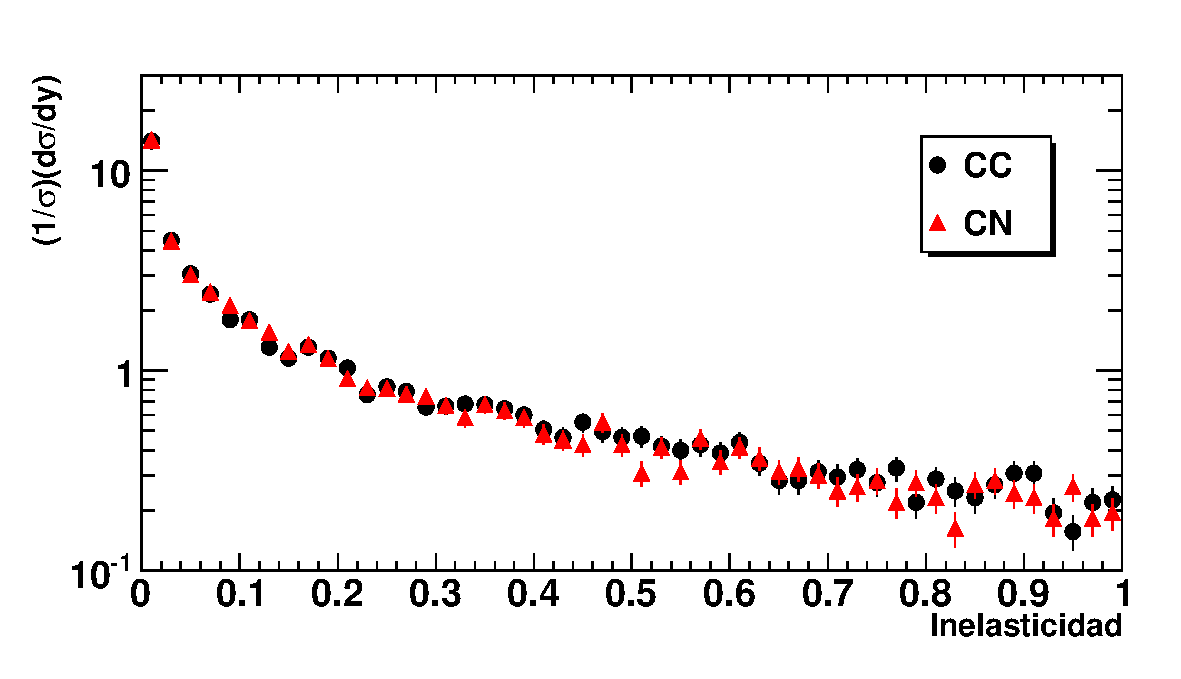
\includegraphics[width=0.80\textwidth]{fig/simulacionAuger/Inelasticity}
	\caption{Comparación de la distribución de inelasticidad para interacciones $\nu$--nucleón de alta energía para CN y CC.}
	\label{fig:inelast}
	\end{center}
	\end{figure}
	%

	El canal $\nu_{\tau}$ vía CC es un caso que requiere un tratamiento más sofisticado. Al igual que el muón, el leptón $\tau$ es una partícula muy penetrante, por lo que puede viajar y alejarse del punto en que fue producido. Por otro lado, su vida media es mucho menor que la del muón por lo que la probabilidad de que decaiga antes de alcanzar la tierra puede no ser despreciable. En la Sec.~\ref{sub:simDB} se describe en detalle la metodología utilizada para simular este tipo de eventos.

	
	\subsection{Decaimiento del \tauon{}: \tauola{}}
	
	Luego de propagarse a trav\'es de la atm\'osfera, el \tauon{} decae generando una gran variedad de part\'iculas secundarias que luego inician la EAS.
	Para generar eventos utilizando la probabilidad de decaimiento a cada canal pueden utilizarse un conjunto de librer\'ias llamadas \tauola{}.
	Estas consisten en varios programas Monte Carlo que implementan decaimientos lept\'onicos y semilept\'onicos.
	Como salida se entrega la topolog\'ia completa del evento, incluyendo neutrinos, resonancias intermedias y la estructura completa de spin durante el desarrollo del decaimiento.
	
	La tabla \ref{tab:tauDecay} muestra los primeros ocho canales de decaimiento del \tauon{} utilizados por \tauola{}.
	\begin{table}[h]
		\begin{center}
		\begin{tabular}{|c|l|l|}
		% \hline
		\hline
		\# &Canal   & Probabilidad (\%) \\
		\hline
		1&$\tau^{-}\rightarrow \pi^{-}\pi^{0}\nu_{\tau}$   & $\sim$25.5 \\
		2&$\tau^{-}\rightarrow e^{-}\bar{\nu_{e}}\nu_{\tau}$   & $\sim$17.9 \\
		3&$\tau^{-}\rightarrow \mu^{-}\bar{\nu_{\mu}}\nu_{\tau}$   & $\sim$17.4 {\bf No genera EAS}\\
		4&$\tau^{-}\rightarrow \pi^{-}\nu_{\tau}$   & $\sim$10.9 \\
		5&$\tau^{-}\rightarrow 2\pi^{-}\pi^{+}\nu_{\tau}$   & $\sim$9.3 \\
		6&$\tau^{-}\rightarrow \pi^{-}2\pi^{0}\nu_{\tau}$   & $\sim$9.3 \\
		7&$\tau^{-}\rightarrow 2\pi^{-}\pi^{+}\pi^{0}\nu_{\tau}$   & $\sim$4.6 \\
		8&$\tau^{-}\rightarrow \pi^{-}3\pi^{0}\nu_{\tau}$   & $\sim$1.0 \\
		\hline
		\end{tabular}
		\end{center}
		% }
		\caption{\label{tab:tauDecay}
		Canales mediante el \tauon{} decae el $\sim96\%$ de los casos. El canal numero 3 no se observa debido a que el $\mu$ generado en el decaimiento escapa sin generar una lluvia atmosférica.
		}
	\end{table}
	Dado que el canal número 3 no genera EAS, dado que el muón escapa sin interactuar, esos eventos no fueron simulados. 
	Para subsanar esto, luego será necesario corregir las eficiencias de trigger e identificación por un factor $0.826$ que tiene en cuenta la falta de este canal.
	
	\section{Desarrollo de las EAS: Aires}

	En la actualidad existen varios programas para simular la formación de una EAS a partir de una partícula primaria a lo largo de la atmósfera terrestre.
	Entre ellos están {\sc corsika}, {\sc aires}, etc.
	En este trabajo se utilizaron EAS simuladas mediante {\sc aires}.

	{\sc Aires} es un conjunto de programas y subrutinas que simulan la lluvia de partículas luego de la incidencia de una rayo cósmico y permite administrar la información relacionada. 

	Este simulador provee un ambiente realista donde la propagación de las partículas se da teniendo en cuanta las características de la atmósfera, el campo geomagnético y la curvatura de la Tierra. 
	
	Debido a que la cantidad de part\'iculas generada en una EAS se vuelve rapidamente inmanejable\footnote{Por ejemplo, para una EAS cuya part\'icula primaria posee \cant{10^{17}}{eV} puede llegar a tener del orden de $10^8$ part\'iculas de energ\'ia mayor a \cant{100}{MeV}. Esto requerir\'ia de orden de \cant{100}{GB} para almacenarlas y 15 d\'ias de tiempo de m\'aquina para seguirlas a todas. Por lo general es necesario simular del orden de $10^3\textit{-}10^4$ EAS para hacer cualquier comparaci\'on con datos experimentales.}, es com\'un en estos programas utilizar un procedimiento estadístico de muestreo llamado {\em thinning}.
	Este consiste en tomar un \textit{set} representativo de part\'iculas que luego es propagado.
	La elecci\'on de dicho set es tal que no se alteran los valores medios de los observables de la lluvia.
	Una explicaci\'on del algoritmo puede encontrarse en \cite{thining}.

	Las partículas que se tienen en cuenta en las simulaciones son: gammas, electrones, positrones, muones, piones, kaones, mesones eta, bariones lambda, nucleones, antinucleones y núcleos de hasta Z=36.
	Los neutrinos electr\'onicos y mu\'onicos que son generados en ciertos decaimientos se tienen en cuenta en cuanto a la energía, pero no son propagados.
	
	La part\'icula que inicia la lluvia puede ser cualquiera de las mencionadas con energías que pueden variar en el rango de \cant{10^9{\it-}10^{21}}{eV}. 
	Tambi\'en es posible simular lluvias iniciadas por partículas primarias ``especiales'' utilizando un módulo que debe escribir cada usuario, capaz de procesar la primer interacción del primario y devolver una lista de part\'iculas tradicional que {\sc aires} pueda aceptar. 

	Los procesos físicos m\'as importantes (desde el punto de vista probabilístico) que las lluvias de part\'iculas pueden sufrir son tenidos en cuenta en las simulaciones. 
	Estos procesos son:

	\begin{itemize}
	\item Procesos electrodin\'amicos: producci\'on de pares y aniquilaciones electr\'on-positr\'on, bremsstrahlung (electrones, positrones y muones), producci\'on de pares mu\'onicos, electrones sacados de \'orbitas at\'omicas (rayos $\delta$), efectos Compton y fotoel\'ectrico, efecto Landau-Pomeranchuk-Migdal (LPM) y supresi\'on diel\'ectrica.
	\item Decaimientos de part\'iculas inestables.
	\item Procesos Hadr\'onicos: colisiones inel\'asticas hadr\'on-n\'ucleo y fot\'on-n\'ucleo, muchas veces simulados utilizando paquetes externos que implementan un modelo de interacci\'on hadr\'onico, como los modelos SIBYLL, QGSJET o QGSJET2, Reacciones fotonucleares, Fragmentaciones nucleares, elásticas e inelásticas.
	\item Propagaci\'on de part\'iculas cargadas: perdidas de energ\'ia en el medio (ionizaci\'on), dispersiones múltiples de Coulomb y deflexiones geomagn\'eticas.
	\end{itemize}    

	Tambi\'en, el sistema de simulación de {\sc aires} provee una plataforma que permite hacer uso del poder de c\'alculo de las computadoras actuales:
	
	\begin{itemize}
	\item Implementa un lenguaje de comandos iniciales (IDL por {\em Input Directive Language}), que consiste en un conjunto simple de comandos que permiten un control eficiente de los par\'ametros de entrada para cada simulación. 
	\item El sistema que lleva a cabo las simulaciones es una herramienta poderosa en plataformas UNIX, ya que permite al usuario coordinar muchas simulaciones en simultaneo, controlar la evolución de un dado trabajo mientras que se está llevando a cabo, etc.
	\item El programa que administra la información de salida procesa archivos generados por el programa principal y permite obtener información relacionada con los observables físicos durante y al final de cada simulación.
	\item Finalmente, hay una librería que provee una serie de rutinas auxiliares para procesar la información generada. En particular, la información m\'as relevante es contenida en archivos comprimidos. \'Esta consiste en informaci\'on detallada de cada part\'icula que llega al piso y de la lluvia en diferentes alturas, que se registra durante la evolución de la misma.
	\end{itemize}
	
	\section{Señal en el detector: Offline}
	
	Una vez la lluvia alcanza el nivel del suelo, es necesario simular la respuesta del detector, para lo que se utiliza \Offline{}.
	Este programa, desarrollado en C++, fue dise\~nado especialmente para cubrir los requerimentos del proyecto Auger. Por ejemplo:
	\begin{itemize}
	\item Contiene una intefaz intuitiva y f\'acil de comprender, que sigue la misma l\'ogica que el detector real.
	\item Dicha interfaz permite acceder a informaci\'on del detector u otros (archivada en diversos formatos) mediante comandos simples y estandarizados.
	\item Es posible cambiar completamente la implementaci\'on de cualquier algoritmo sin cambiar en absoluto la interfaz.
	\item Es posible simular un detector completamente heterog\'eneo en el que cada tanque o telescopio tiene identidad propia.
	\item El grado de detalle con el que se realizan las simulaciones puede variar f\'acilmente, seg\'un se necesite.
	\end{itemize}
	
	\subsection{Algoritmos dentro de Offline}
	
	Si bien \Offline{} posee una gran cantidad de algoritmos que se utilizan en diferentes \'areas dentro de la colaboraci\'on, aqu\'i s\'olo se introducen unos pocos que son importantes en este an\'alisis.
	
		\subsubsection{Unthinning}
		
		Una vez que la EAS alcanza el nivel del suelo, las part\'iculas presentes se guardan, por lo general, en archivos binarios en diversos formatos, que dependen del simulador empleado.
		Si se ha utilizado un algoritmo de thinning, cada part\'icula se guarda con un peso respectivo que hace referencia a la cantidad de part\'iculas que esta representa.
		\Offline{} no s\'olo permite leer archivos provenientes de varios simuladores (entre los que se encuentra {\sc Aires}), sino que tambi\'en aplica un algoritmo de \textit{unuhinning} de manera de regenerar las part\'iculas no simuladas y tenerlas en cuenta en la se\~nal sobre el detector.
		
		Dado que el \'area instrumentada a nivel del suelo es muy chica y s\'olo unas pocas de las part\'iculas que llegan a este nivel interactuan con el detector,
% 		Por este motivo, para realizar el \textit{unthinning}, 
		\Offline{} realiza el unthinning utilizando un \textit{m\'etodo de muestreo local}.
		Todas las part\'iculas dentro de cierta zona de muestreo (correspondiente a cada detector) son seleccionadas.
		Luego, se las dispersa espacial y temporalmente utilizando un m\'etodo estad\'istico, que se describe en \cite{unthinning1}.
		
		Una vez que las part\'iculas, clones de la primaria, son dispersadas se las inyecta en posiciones aleatorias de la pared del detector, teniendo en cuenta la direcci\'on de incidencia. 
		Un ejemplo de esto \'ultimo se muestra en la figura \ref{fig:unthinning_tank}.
		%
		\begin{figure}[h!]
			\begin{center}
			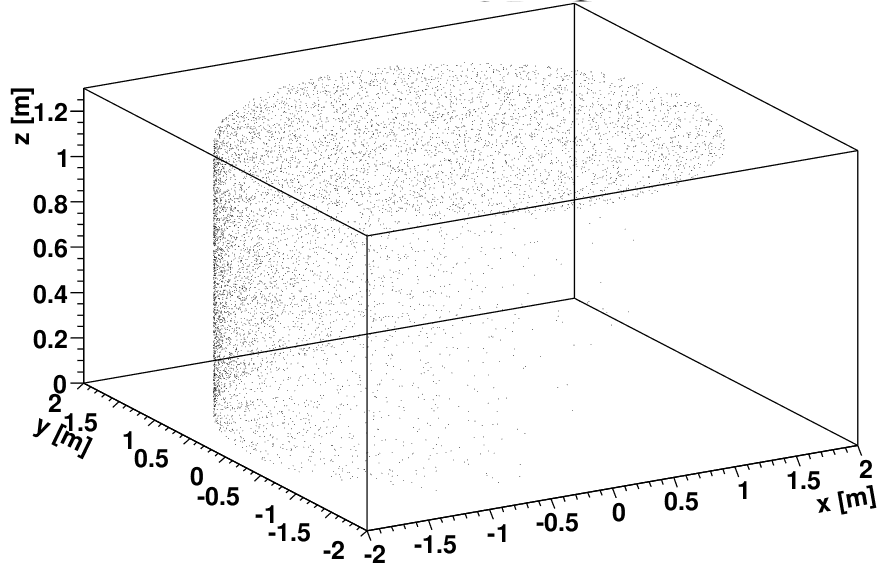
\includegraphics[width=0.7\textwidth]{fig/simulacionAuger/unthinning_tank}
			\caption{Distribuci\'on de part\'iculas sobre la superficie de un tanque luego de aplicar el algoritmo de unthinning.}
			\label{fig:unthinning_tank}
			\end{center}
		\end{figure}
		%
		
		En particular, el algoritmo de unthinning no es directamente aplicable a lluvias rasantes a la tierra, por lo que una modificaci\'on del mismo se incluye en \Offline{} con el fin de resolver sus problemas.
		
% 		\textbf{RECTANGULOS ??}
		
		\subsubsection{Simulaci\'on del tanque}
		
		Para simular la respuesta del detector de superficie se ha incorporado en \Offline{} un m\'odulo especializado en la simulaci\'on del tanque basado en {\sc geant 4}~\cite{geant4}.
		
		{\sc geant 4} consiste en una librer\'ia de C++ que provee las herramientas necesarias para simular tanto la f\'isica como la geometr\'ia del detector.
		Algunas caracter\'isticas de dise\~no se exponen a continuaci\'on:
		\begin{itemize}
		\item Se procur\'o que todos los aspectos f\'isicos en esta etapa de la simulaci\'on sean lo m\'as precisos posible, mientras se trat\'o de tener buen entendimiento de su influencia en el resultado final.
		\item Por ser {\sc geant 4} una versi\'on m\'as sofisticada de programas anteriores, algunas de las variables del tanque fueron ajustadas de tal forma que los resultados experimentales se reproduzcan\footnote{Una de las m\'as importantes es la cantidad de fotoelectrones detectados por mu\'on vertical incidente.}.
		\item La velocidad de simulaci\'on es un factor importante.
		La simulaci\'on de estaciones cercanas al centro de la lluvia puede ser muy costosa debido a la gran cantidad de part\'iculas que se generan en esa regi\'on. Para evitar este inconveniente, se aplican cortes espec\'ificos en la producci\'on de fotones en el seguimiento de muones.
		\end{itemize}
		
		Por otro lado, a continuaci\'on se especifican algunos de los procesos f\'isicos tenidos en cuenta en la simulaci\'on del tanque:
		%
		\begin{itemize}
		\item La simulaci\'on de la propagaci\'on de una part\'icula cargada puede incluir efectos de ionizaci\'on, producci\'on de rayos delta, scattering de Coulomb multiple, bremsstrahlung y radiaci\'on Cherenkov.
		\item Lor fotones producidos en la radiaci\'on Cherenkov (incluyendo los producidos por los rayos delta) son sometidos a scattering de Rayleigh, absorci\'on e interacci\'on \'optica con las paredes del tanque. La polarizaci\'on del fot\'on es tenida en cuenta siempre que es relevante.
		\end{itemize}
		%
		En particular, se encuentran especialmente modeladas y optimizadas las propiedades \'opticas de Tyvek, la longitud de absorci\'on del agua y la geometr\'ia de los PMTs.
		En la figura \ref{fig:cher_tank_sim} se muestra la simulaci\'on de los fotones Cherenkov generados en el pasaje de un electr\'on de baja energ\'ia a trav\'es del tanque.
		%
		\begin{figure}[h!]
			\begin{center}
			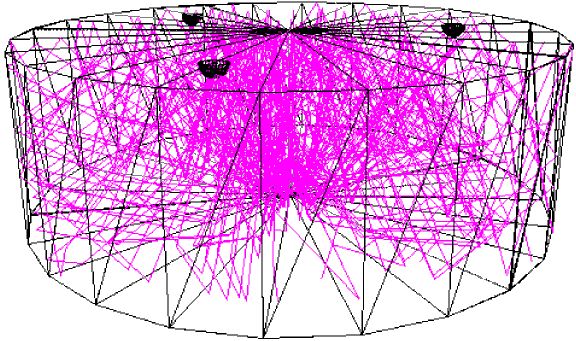
\includegraphics[width=0.7\textwidth]{fig/simulacionAuger/cher_tank_sim}
			\caption{Simulaci\'on de fotones Cherenkov generados en el pasaje de un electron de baja energ\'ia a trav\'es del tanque.}
			\label{fig:cher_tank_sim}
			\end{center}
		\end{figure}
		%
		
		Adem\'as de toda la f\'isica involucrada, la electr\'onica de la estaci\'on tambien es simulada.
		Luego de esta etapa, cada tanque involucrado en un evento tiene sus trazas FADC calculadas listas para ser analizadas por los algoritmos de trigger.
		
		\subsubsection{Trigger}
		
		Una vez que las trazas FADC fueron calculadas, \Offline{} posee algoritmos que calculan cada nivel de trigger del detector, desde disparos locales T2 hasta CDAS T4 y T5, especificados en la secci\'on \ref{sbsc:trig_levels}.
		
		
	\section{Librería de eventos}
	
	Finalmente, para cada búsqueda se simuló una librería de eventos que cubra todo el espacio de parámetros en el cual se esperan neutrinos y que a su vez puedan generar lluvias que disparen el detector.
	
	\subsection{Eventos DGL}
	
	Para el canal CC se utilizaron energías fijas entre \cant{10^{17}}{eV} y \cant{10^{20.5}}{eV} con un paso logarítmico de $0.5$. Dado que el canal NC sólo lleva el $20\%$ de la energía del neutrino, el rango energético fue acortado a \cant{10^{18}\ -\ 10^{20.5}}{eV}, evitando así simular eventos que no dispararían el detector.
	En canal double bang no fue tenido en cuenta, por lo que las lluvias iniciadas por \nutau{} se simularon como NC.
	En ambos canales, se simularon ángulos cenitales desde $60^\circ$ a $75^\circ$ con un paso de $3^\circ$, utilizando ángulos azimutales aleatorios entre $0^\circ$ y $360^\circ$.
	Con el fin de maximizar la eficiancia a la hoa de simular se forzó a los neutrinos a interactuar en puntos de inyección de profundidad $D$, uniformemente distribuidos entre un máximo y un mínimo (que dependen del ángulo cenital) con un paso fijo de \cant{100}{g cm^{-2}}.
	Algunos puntos de inyección muy cercanos al suelo fueron omitidos debido a que la lluvia no llega a desarrollarse lo suficiente como para dar trigger.
	Para cada punto ($E_{\nu}$, $\theta$, $D$) se generaron 50 cascadas atmosféricas independientes.
	Cada una de estas se utilizó para producir cinco eventos con diferente punto de impacto en \Offline{}, dando un total de 250 eventos cuasi-independientes para cada punto de inyección.
	Todo lo anterior se resume en la tabla \ref{tab:sim_table_dgl}, mientras que la figura \ref{fig:sim_fig_dgl} muestra las profundidades simuladas como función del ángulo cenital.
	
	\begin{table}[ht]
		\begin{center}
		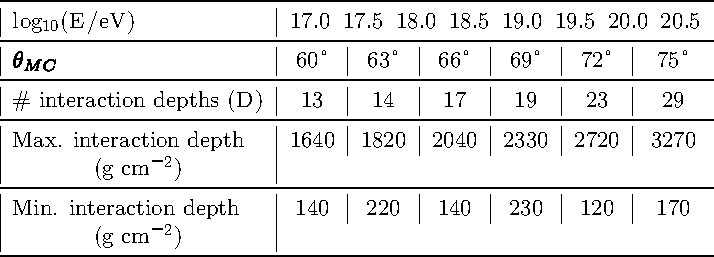
\includegraphics[width=0.85\textwidth]{fig/simulacionAuger/simShNavarro_1}
		\end{center}
		\caption{Resumen de las energías, ángulos cenitales y puntos de inyección. Para cada angulo, se simuló un número determinado de profundidades de interacción entre el máximo y un mínimo especificado en la tabla, con un paso de \cant{100}{g cm^{-2}}. Los dos primeros bines de energía no fueron simulados para el canal NC.
		}
		\label{tab:sim_table_dgl}
	\end{table}
	%
	\begin{figure}[h!]
		\begin{center}
		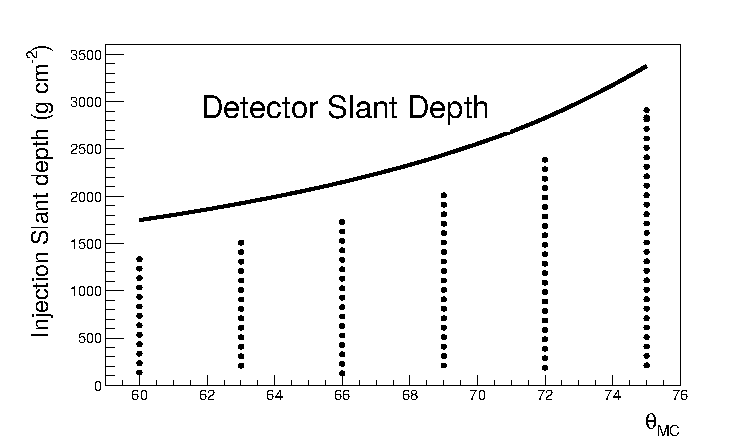
\includegraphics[width=0.85\textwidth]{fig/simulacionAuger/simShNavarro_2}\\
		\caption{En linea llena se grafica la prufundidad atmoférica inclinada del Observatorio Pierre Auger, que se encuentra a \cant{1400}{m} sobre el nivel del mar.
		Los circulos indican los puntos de inyección de los neutrinos (puntos de interacción) para diferentes ángulos cenitales.
		}
		\label{fig:sim_fig_dgl}
		\end{center}
	\end{figure}
	
	
	\subsection{Eventos DGH}
	
	La librería de eventos DGH fue obtenida con criterios muy similares a los utilizados en DGL, con la salvedad de que en este canal si se tuvieron en cuenta los eventos double bang.
	La Tab.~\ref{tab:sim_table_dgh} resume el conjunto de simulaciones producidas para este rango angular.
	\begin{table}[ht]
	\begin{center}
	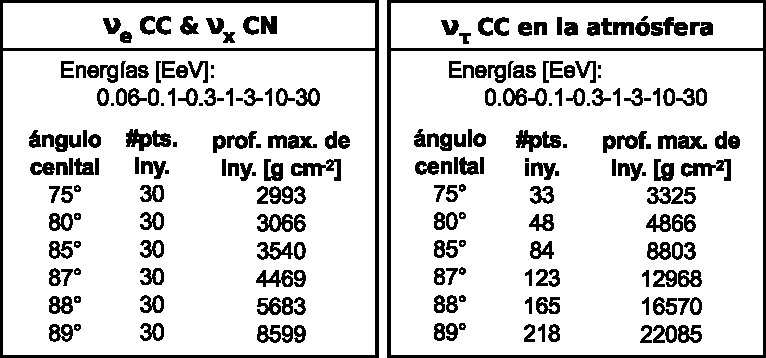
\includegraphics[width=0.85\textwidth]{fig/simulacionAuger/sim_table.pdf}
	\end{center}
	\caption{
	Resumen, discriminado por canal de interacción, de las simulaciones de neutrinos profundos realizadas.
	Para cada ángulo cenital se indica la profundidad de inyección máxima considerada (medida inclinada desde el detector) y la cantidad de puntos de inyección simulados en este rango. Las energías indicadas corresponden a la del neutrino primario.
	}
	\label{tab:sim_table_dgh}
	\end{table}
	Para cada ángulo cenital se indica la profundidad de inyección máxima considerada (medida inclinada desde el detector) y la cantidad de puntos de inyección simulados en este rango. Las energías indicadas corresponden a la del neutrino primario.
	
	\subsection{Eventos ES}
	
	En el caso de los eventos ES los parámetros que identifican una lluvia atmosférica son el ángulo cenital $\theta$, el ángulo azimutal $\Phi$, la energía del \tauon{} que escapa de la tierra \etau{} y la altura sobre el detector a la que el \tauon{} decae \xd{}.
	La energía del \tauon{} cubrió valores entre \cant{10^{16.5}}{eV} hasta \cant{10^{19.5}}{eV}, con paso de 0.5 logarítmico salvo en la zona de baja energía cuyo paso fue de 0.25.
	El ángulo cenital barrió valores desde $90.111^\circ$ hasta $95.884^\circ$ con paso de $0.573^\circ=0.1 \rm rad$ y en la zona de baja energía el ángulo máximo fue en algunos casos $93.549^\circ$.
	El ángulo azimutal $\Phi$ se eligió al azar entre $0^\circ$ y $360^\circ$.
	Con respecto a la altura de decaimiento \xd{} se utilizó un valor máximo que dependió de la energía del \tauon, y pasos de \cant{100}{m} o \cant{50}{m} para la zona de baja energía.
	Al igual que para los eventos DGH, para generar la libreria de eventos ES se simularon 50 eventos para cada punto ($\theta$,\etau{},\xd{}) y se utilizó cada lluvia 3 veces sobre el detector, logrando 150 eventos cuasi-independientes en cada caso. 
	La tabla \ref{tab:sim_table_es} condensa toda la información sobre las simulaciones ES, mientras que la figura \ref{fig:sim_fig_es} muestra los conjuntos de ($\theta$,\etau{},\xd{}) simulados.
	%
	\begin{table}
		\begin{center}
		\footnotesize
			\begin{tabular}{|c|c|cc|cc|}
			\hline
			\makebox[0.1\textwidth][c]{Group} & \makebox[0.13\textwidth][c]{\etau{} [eV]}&
			\makebox[0.15\textwidth][c]{\tita{} Min - Max} & \makebox[0.07\textwidth][c]{step [º]} & \makebox[0.13\textwidth][c]{\xd{} Min - Max} & \makebox[0.07\textwidth][c]{step [m]}\\
			\hline
			\hline
			\multirow{2}{*}{E003EeV} & \multirow{2}{*}{$3.16\times10^{16}$} & $95.884\text{ - }90.111$ & $0.573$ & $0\text{ - }600$ & $100$\\
			& & $93.549\text{ - }90.111$ & $0.573$ & $0\text{ - }300$ & $50$\\
			
			\multirow{2}{*}{E006EeV} & \multirow{2}{*}{$5.62\times10^{16}$} & \multirow{2}{*}{$93.549\text{ - }90.111$}  & \multirow{2}{*}{$0.573$} & \multirow{2}{*}{$0\text{ - }300$} & \multirow{2}{*}{$50$}\\
			& & & & &\\
			
			\multirow{2}{*}{E01EeV} & \multirow{2}{*}{$10^{17}$} & $95.884\text{ - }90.111$ & $0.573$ & $0\text{ - }700$ & $100$\\
			& & $93.549\text{ - }90.111$ & $0.573$ & $0\text{ - }300$ & $50$\\
			
			\multirow{2}{*}{E02EeV} & \multirow{2}{*}{$1.78\times10^{17}$} & \multirow{2}{*}{$93.549\text{ - }90.111$}  & \multirow{2}{*}{$0.573$} & \multirow{2}{*}{$0\text{ - }300$} & \multirow{2}{*}{$50$} \\
			& & & & &\\
			
			\multirow{2}{*}{E03EeV} & \multirow{2}{*}{$3.16\times10^{17}$} & $95.884\text{ - }90.111$ & $0.573$ & $0\text{ - }1000$ & $100$\\
			& & $93.549\text{ - }90.111$ & $0.573$ & $0\text{ - }300$ & $50$\\
			
			\multirow{2}{*}{E06EeV} & \multirow{2}{*}{$5.62\times10^{17}$} & \multirow{2}{*}{$93.549\text{ - }90.111$}  & \multirow{2}{*}{$0.573$} & \multirow{2}{*}{$0\text{ - }300$} & \multirow{2}{*}{$50$}\\
			& & & & & \\
			
			\multirow{2}{*}{E1EeV} & \multirow{2}{*}{$10^{18}$} & $95.884\text{ - }90.111$ & $0.573$ & $0\text{ - }1400$ & $100$ \\
			& & $93.549\text{ - }90.111$ & $0.573$ & $0\text{ - }300$ & $50$ \\
			
			\multirow{2}{*}{E3EeV} & \multirow{2}{*}{$3.16\times10^{18}$} & \multirow{2}{*}{$95.884\text{ - }90.111$}  & \multirow{2}{*}{$0.573$} & \multirow{2}{*}{$0\text{ - }1300$} & \multirow{2}{*}{$100$}\\
			& & & & & \\
			
			\multirow{2}{*}{E10EeV} & \multirow{2}{*}{$10^{19}$} & \multirow{2}{*}{$95.884\text{ - }90.111$}  & \multirow{2}{*}{$0.573$} & \multirow{2}{*}{$0\text{ - }1300$} & \multirow{2}{*}{$100$} \\
			& & & & & \\
			
			\multirow{2}{*}{E30EeV} & \multirow{2}{*}{$10^{19.5}$} & \multirow{2}{*}{$95.884\text{ - }90.111$}  & \multirow{2}{*}{$0.573$} & \multirow{2}{*}{$0\text{ - }2500$} & \multirow{2}{*}{$100$} \\
			& & & & &\\
			\hline
			\end{tabular}
		\end{center}
		\caption{\label{tab:sim_table_es}
		Detalle de los parámetros utilizados para generar la librería de eventos ES.
		}
	\end{table}
	%
	\begin{figure}[h!]
		\begin{center}
		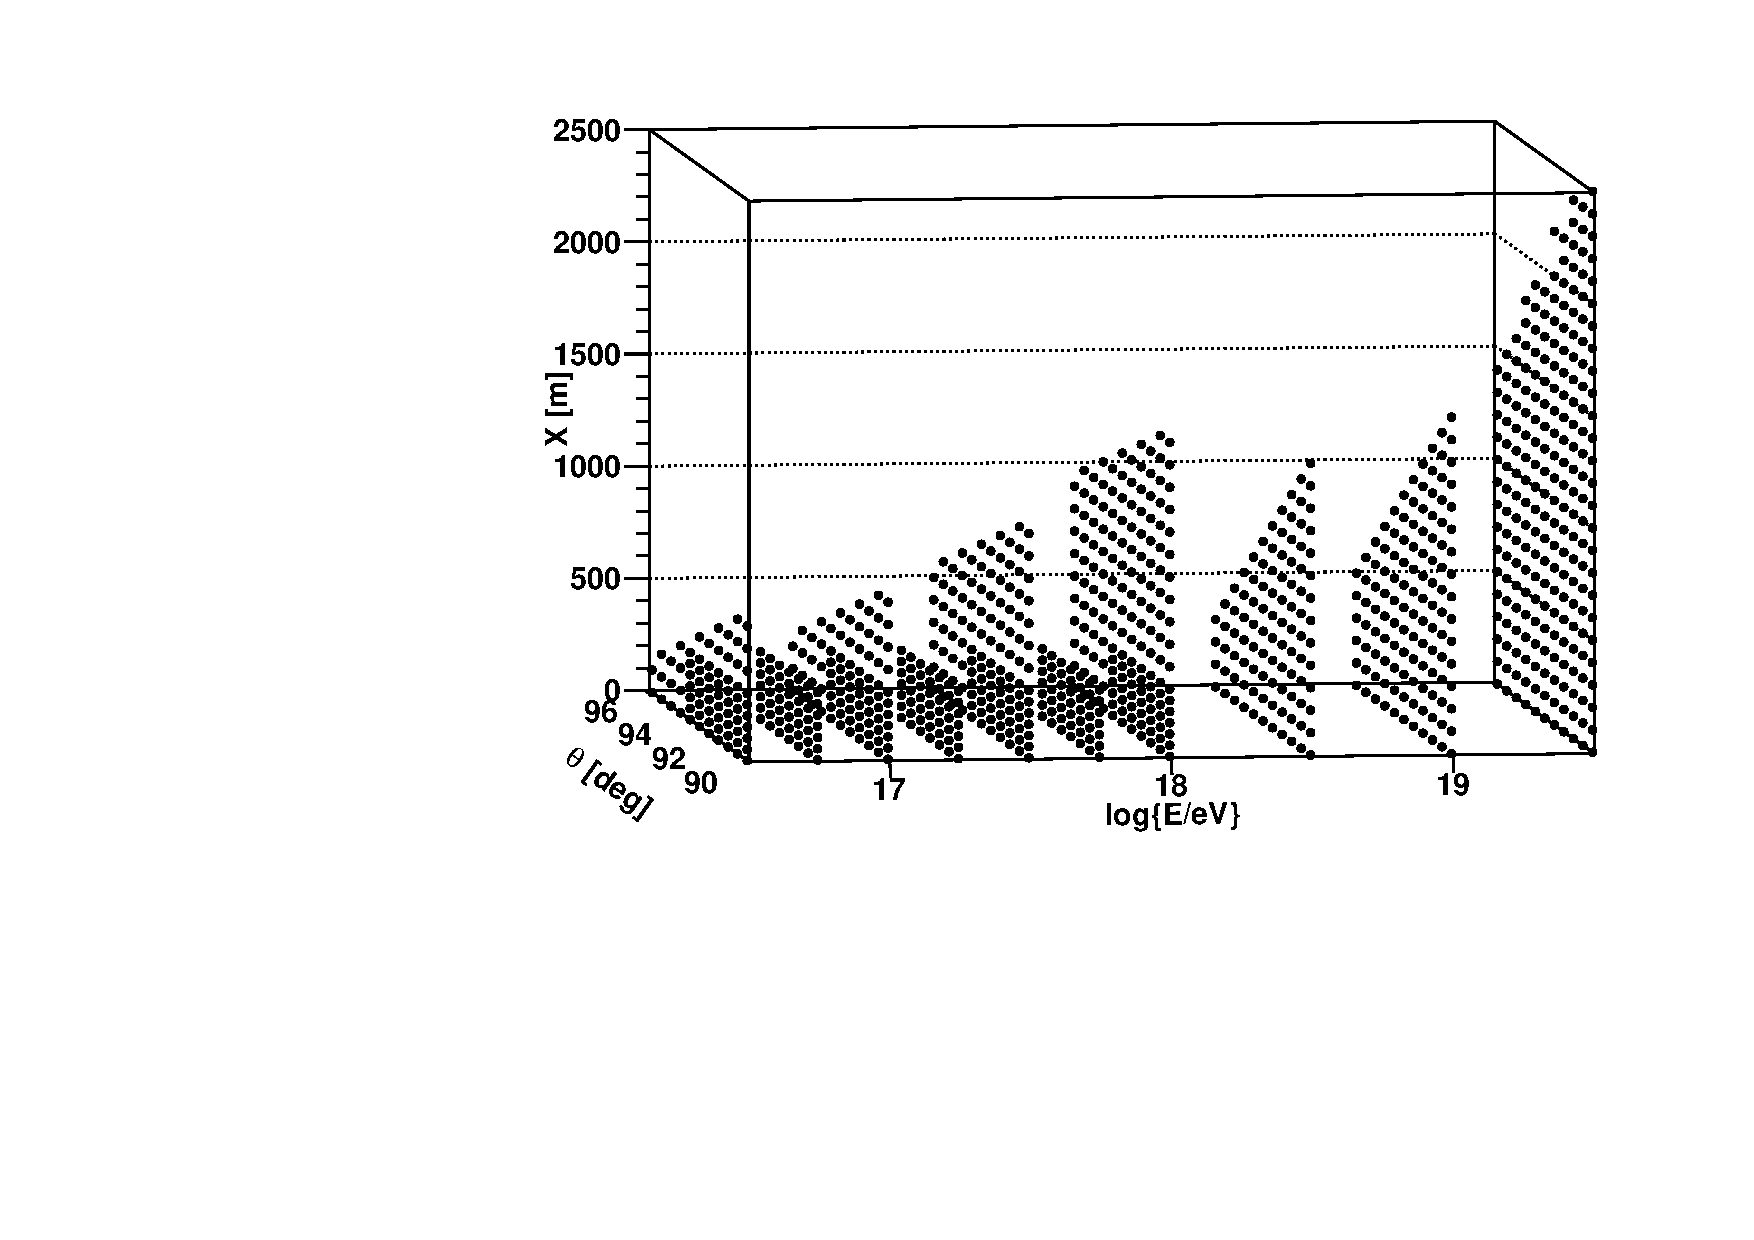
\includegraphics[width=0.85\textwidth]{fig/simulacionAuger/3D_completeParameterSpace5}
		\caption{
		Conjunto de ($\theta$,\etau{},\xd{}) utilizados para generar la librería de eventos ES.
		}
		\label{fig:sim_fig_es}
		\end{center}
	\end{figure}
	